\documentclass[{../../master}]{subfiles}
\graphicspath{{../..}}  % 個別コンパイル時の画像パスを解決する

\begin{document}

\section{\textsf{caster\_*\_link}の作成と追加}

ロボットのモデルに自在キャスターを追加しましょう.
実機用のモデルには必要のないリンクですが,後々シミュレーションを行うときに必要になるので,今のうちに追加しておきます.

自在キャスターは2つのパーツから構成されます.
1つ目はキャスターの車輪パーツ,2つ目は車輪を支えるサポートパーツです.
シミュレーションを行うことを考えて,これらのパーツを別々のリンクとして定義することにします.

\subsection{\textsf{caster.xacro}の作成}

\textsf{urdf/}ディレクトリ以下に\textsf{caster/}ディレクトリを作り,その中に\textsf{caster.xacro}という名前のファイルを作成します.
そして,コード\ref{code:caster_link_xacro}の内容を記述します.

\begin{lstlisting}[language=XML, label=code:caster_link_xacro, caption=\textsf{caster.xacro}]
<?xml version="1.0"?>
<robot xmlns:xacro="http://ros.org/wiki/xacro">
  <xacro:macro name="caster" params="prefix parent *joint_origin">
    <joint name="${prefix}_caster_support_joint" type="fixed">
      <xacro:insert_block name="joint_origin"/>
      <parent link="${parent}"/>
      <child link="${prefix}_caster_support_link"/>
    </joint>
    
    <link name="${prefix}_caster_support_link">
      <visual>
        <origin rpy="0.0 0.0 0.0"/>
        <geometry>
          <mesh filename="package://adamr2_description/meshes/caster_support_link.STL"/>
        </geometry>
        <material name="red">
          <color rgba="0.0 0.0 0.0 1.0"/>
        </material>
      </visual>
    </link>

    <joint name="${prefix}_caster_wheel_joint" type="fixed">
      <origin xyz="-0.030 0.0 -0.072" rpy="0.0 0.0 0.0"/>
      <parent link="${prefix}_caster_support_link"/>
      <child link="${prefix}_caster_wheel_link"/>
    </joint>

    <link name="${prefix}_caster_wheel_link">
      <visual>
        <origin rpy="0.0 0.0 0.0"/>
        <geometry>
          <mesh filename="package://adamr2_description/meshes/caster_wheel_link.STL"/>
        </geometry>
        <material name="red">
          <color rgba="0.0 0.0 0.0 1.0"/>
        </material>
      </visual>
    </link>
  </xacro:macro>
</robot>
\end{lstlisting}

\textsf{caster.xacro}では,\textsf{\$\{prefix\}\_caster\_support\_link}と\textsf{\$\{prefix\}\_caster\_wheel\_link}の2つのリンクと,それらを繋ぐ\textsf{\$\{prefix\}\_caster\_support\_joint}と\textsf{\$\{prefix\}\_caster\_wheel\_joint}の2つのジョイントを定義するマクロ\textsf{caster}を定義しています.
\textsf{caster}マクロは3つの引数を取ります.
このうち,\textsf{prefix}はリンクやジョイントの名前の接頭辞です.
自在キャスターはロボットの前後に1つずつ存在しますが,それらは全く同じパーツなので,xacroファイルを複数定義するのは無駄になります.
そのため,接頭辞を引数にとって区別することで,1つのxacroファイルで2つの部品を定義できるようにしています.

\textsf{base\_link}と\textsf{\$\{prefix\}\_caster\_support\_link}は\textsf{\$\{prefix\}\_caster\_support\_joint}によって接続されます.
ジョイントタイプは\textsf{fixed}です.
本来ならばこのジョイントは,Z軸を回転中心とする連続回転ジョイントのタイプにする必要があります.
しかし,実機用のURDFファイルでこのような受動回転するコンポーネントのジョイントタイプを連続回転にすると,リンクの位置関係を取得できないためにTFのエラーが発生します.
そのため,実機用URDFではジョイントのタイプを\textsf{fixed}にしています
.
\textsf{\$\{prefix\}\_caster\_support\_link}と\textsf{\$\{prefix\}\_caster\_wheel\_link}を繋ぐジョイント\textsf{\$\{prefix\}\_caster\_wheel\_joint}も同様に固定タイプのジョイントとしています.

サポートパーツと車輪パーツの位置関係は一定なので,xacroファイル内でローカルに\textsf{\$\{prefix\}\_caster\_wheel\_joint}の原点を設定してしまっています.
一方で,自在キャスターがロボットボディのどこに取り付けられるかはユーザー次第なので,\textsf{\$\{prefix\}\_caster\_support\_joint}の原点はルートファイルから決定できるように,マクロのブロックパラメータとして設定しています.

\subsection{STLファイルの作成と割り当て}

\ref{sec:base_link_create_mesh_file}を参考に,3D-CADソフトからSTLファイルをエクスポートして\textsf{meshes/}ディレクトリに配置してください.
車輪パーツとサポートパーツは別ファイルとして書き出します.
出力座標系は図\ref{fig:caster_link_coordinate}を参照してください.

\begin{figure}[ht]
  \centering
  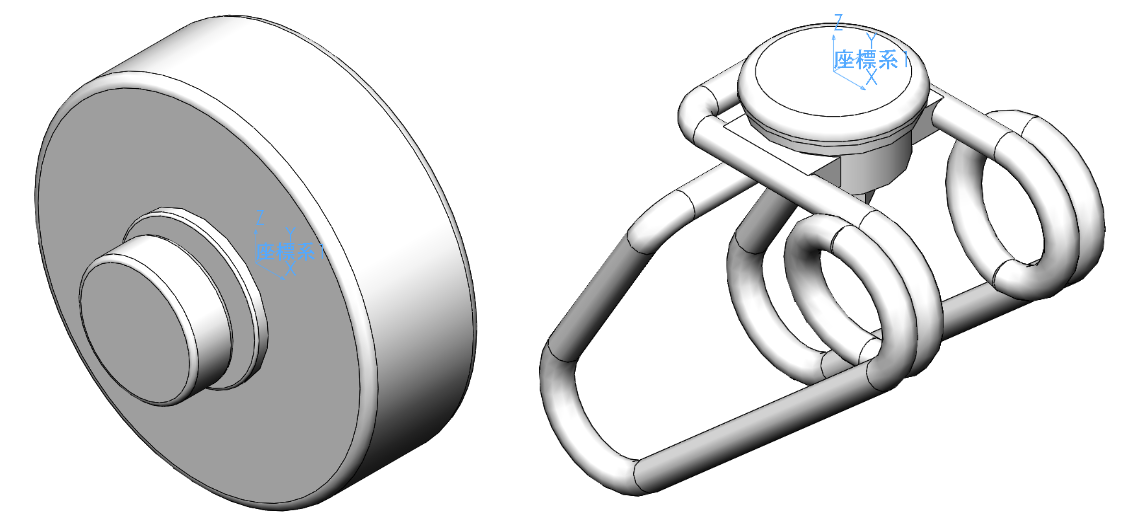
\includegraphics[height=40truemm]{images/caster_link_coordinate.drawio.png}
  \label{fig:caster_link_coordinate}
  \caption{Coordinate System of Caster Parts}
\end{figure}


\subsection{ルートファイルからインクルードする}

作成したリンクをロボットモデルに組み込みましょう.\textsf{robot.xacro}にコード\ref{code:robot_xacro_add_caster_link}のように追記します.

\begin{lstlisting}[language=XML, label=code:robot_xacro_add_caster_link, caption=Add Caster-Link to Robot Model]
<?xml version="1.0"?>
<robot name="adamr2" xmlns:xacro="http://ros.org/wiki/xacro">
  <xacro:include filename="$(find adamr2_description)/urdf/base/base.xacro"/>
  <xacro:include filename="$(find adamr2_description)/urdf/caster/caster.xacro"/>

  <link name="base_footprint"/>

  <xacro:base parent="base_footprint">
    <origin xyz="0.0 0.0 0.262"/>
  </xacro:base>

  <xacro:caster prefix="back" parent="base_link">
    <origin xyz="-0.275 0.0 -0.1498"/>
  </xacro:caster>

  <xacro:caster prefix="front" parent="base_link">
    <origin xyz="0.275 0.0 -0.1498" rpy="0 0 ${radians(180)}"/>
  </xacro:caster>
</robot>
\end{lstlisting}

\textsf{caster.xacro}ファイルをインクルードし,\textsf{xacro:caster}マクロを使って前後の自在キャスターを定義しています.
ロボットの前方に付けるキャスターは,向きを180度変えるために\textsf{origin}要素の\textsf{rpy}属性でヨー角を設定しています.

\end{document}